\documentclass[a4paper,10pt]{article}
\usepackage[top=3cm, bottom=3cm, left=3cm, right=3cm]{geometry}
\usepackage[spanish]{babel}
\spanishdecimal{.}
\selectlanguage{spanish}
\usepackage[spanish,onelanguage,ruled]{algorithm2e}
\usepackage[utf8]{inputenc}
\usepackage{graphicx}
\usepackage{caption}
\usepackage{subcaption}
\usepackage{hyperref}
\usepackage{verbatim}
\usepackage{amssymb}
\usepackage{mathtools}
\usepackage{amsmath}
\usepackage[natbibapa]{apacite}
\bibliographystyle{apacite}
%\usepackage[nottoc,numbib]{tocbibind}
\newcommand\ddfrac[2]{\frac{\displaystyle #1}{\displaystyle #2}}
\DeclareMathOperator{\atantwo}{atan2}

\title{Posiciones de los Planetas y la Luna \\ Macroproyecto para Matemáticas}
\author{Marco Negrete, Javier Alatorre, Daniela Madrigal y Melissa Santoyo}
\date{Proyecto Aleph 5}

\begin{document}
\renewcommand{\tablename}{Tabla}
\renewcommand{\BOthers}[1]{et al.\hbox{}}
\maketitle

\begin{abstract}
  Este documento contiene un resumen de los cálculos necesarios para estimar las posiciones de los primeros cinco planetas del sistema solar y la luna, vistos desde un punto dado sobre la Tierra, en una fecha y hora determinadas. También se incluyen instrucciones para escribir el código necesario, en los lenguajes Java y Python, para implementar estos cálculos en la aplicación StarGazer (para Android). La intención de este documento es servir de ayuda en al ejecución de la secuencia didáctica de este macroproyecto. 
\end{abstract}

\section{Cálculo de la posición de los planetas}
Para este macroproyecto se considera que el movimiento de los planetas es Kepleriano, es decir, se considera que la órbita de los planetas es eclíptica y que su movimiento está determinado sólamente por la interacción gravitatoria entre el planeta en cuestión y el sol. Existen factores que alteran el movimiento de un planeta, como la gravedad de otros planetas y la presión de radiación solar, sin embargo, estos efectos son mínimos y para este macroproyecto no se tomaron en cuenta. 

Dados los supuestos anteriores, la posición de un planeta se puede estimar, a grandes rasgos, con los siguientes pasos:
\begin{enumerate}
\item Obtención de los parámetros orbitales (ya sea del sol, los planetas o la Luna).
\item Cálculo de la posición del planeta con respecto al plano de su propia órbita.
\item Transformación de esta posición a coordenadas ecuatoriales.
\item Cálculo del tiempo sideral local.
\item Transformación de coordenadas ecuatoriales a coordenadas horizontales.
\end{enumerate}

Cada uno de los pasos anteriores corresponde a un día de trabajo en al secuencia didáctica. En las siguientes secciones se explican a detalle cada uno de estos cálculos.

\section{Parámetros orbitales}
Para definir qué son los parámetros orbitales, primero es necesario definir algunos sistemas de referencia. El primero de ellos es el sistema de coordenadas eclípticas. En este sistema, el plano $XY$ coincide con el plano de la órbita de la Tierra y el eje positivo de las $X$ apunta hacia el equinoccio vernal, es decir, hacia el punto en el que se encuentra la Tierra, con respecto al sol, cuando ocurre el equinoccio de primavera en el hemisferio norte. En la figura \ref{fig:EclipticFrame} se muestra este sistema de coordenadas. En el sistema eclíptico, el origen puede fijarse en el Sol o en la Tierra, pero el plano $XY$ siempre coincide con el plano orbital de la Tierra y el eje $X$ apunta hacia el Primer Punto de Aries (como también se conoce la dirección en que se encuentra la Tierra en el equinoccio vernal). Lo más común, es utilizar el Sol como origen del sistema eclíptico. 
\begin{figure}
  \centering
  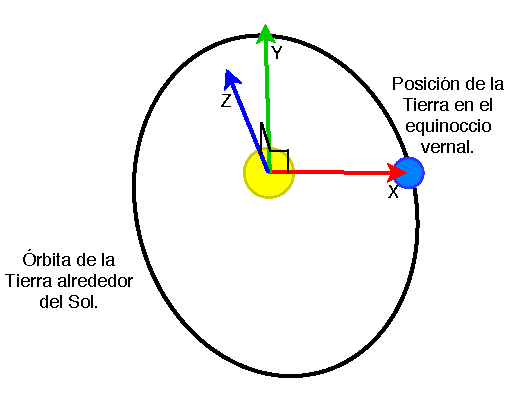
\includegraphics[width=0.5\textwidth]{Figures/EclipticCoordinates.pdf}
  \caption{Sistema de coordenadas eclípticas.}
  \label{fig:EclipticFrame}
\end{figure}

Ahora, las órbitas de todos los planetas son elipses con el Sol en uno de los focos, sin embargo, estas elipses no son coplanares con la órbita de la Tierra, no tienen la misma orientación en el espacio ni la misma ``forma'' y tamaño. Por ello se requieren tres parámetros (ángulos) para definir la orientación de la órbita en el espacio y dos más para definir su forma (qué tanto se parece a un círculo) y tamaño. Una vez definida la forma y orientación de la órbita, un sexto parámetro se utiliza para definir la posición del planeta en un momento determinado. Estos seis parámetros son conocidos como los parámetros orbitates. A continuación se describien más a detalle cada uno de ellos.  
\end{document}